% TeX root = main.tex

% First argument to \section is the title that will go in the table of contents. Second argument is the title that will be printed on the page.
\section[Lecture 2--{Curves}]{2. Curves}
A curve in manifold means either a parameterized curve, i.e., a smooth map $c: [a,b]\rightarrow M$, 
or a set of points in $M$ that is the image of this map.
This section focus on the plane curve, first introduces the regular curves whose velocity never zero
so that can be reparameterized
by arc length. We can define the signed curvature by the second derivative of 
this parameterization.
\subsection{Regular Curves}
\begin{definition}[Regular curve]
    A parameterized curve $c: [a, b] \rightarrow M$ is \textbf{regular}
     if its velocity $c'(t)\neq 0$ for all $t$ in $[a, b]$, which means an immersion from
     $[a, b]$ to $M$.
\end{definition}
\begin{example}
    The curve $c(t)=(t^3, t^2), t\in [-1, 1]$ in $\sR^2$ is not regular since $c'(t)$ is zero
    at $t=0$. 
    Although $c$ is smooth, but the image of $c$ is not smooth as shown 
    in Figure~\ref{fig. t3t2 image}.
\end{example}
\begin{figure}[htb]
    \centering
    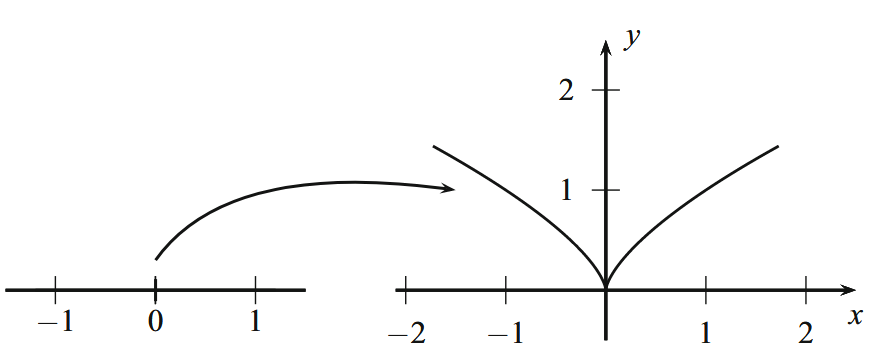
\includegraphics[width=0.7\textwidth]{../Lectures/Figures/curv_image.png}
    \caption{A nonregular curve~\cite[p.~9]{tuDifferentialGeometry2017}.}
    \label{fig. t3t2 image}
\end{figure}
\subsection{Arc Length Parameterization}
The most important \textbf{reparameterization} ($\beta(u):=c(t(u))$ if $t=t(u)$ 
is a diffeomorphism from one to another closed interval) 
is the \textbf{arc length reparameterization}.
We define the \textbf{speed} of a curve $c: [a,b]\rightarrow M$ is $\norm{c'(t)}$, and the
arc length is
\begin{align}
    \ell = \int_{a}^{b} \norm{c'(t)}dt. \nonumber
\end{align}
Then, the \textbf{arc length function} $s: [a, b] \rightarrow [0, \ell]$ of $c$ is
\begin{align}
    s(t)=\int_{a}^{t} \norm{c'(u)}du. \nonumber
\end{align}
\begin{proposition}
    The arc length function $s$ of a regular curve has a $C^\infty$ inverse.
\end{proposition}
\begin{proof}
    The regular property gaurantees $s'(t)=\norm{c'(t)} > 0$, which means $s(t)$ 
    is monotonically increasing, so $t(s)$ is a $C^\infty$ function.
\end{proof}
Thus, we can write the \textbf{arc length reparameterization} of a regular curve
 by $\gamma(s)=c(t(s))$.
\begin{proposition}
    A curve $\gamma(s)$ is reparameterized by arc length if and only if it has \textbf{unit speed} and
    its parameter starts at $0$.
\end{proposition}
\begin{proof}
    $(\Rightarrow)$: as $\gamma(s)=c(t(s))$, the speed is
    \begin{align}
        \norm{\frac{d\gamma}{ds}} = \norm{\frac{dc}{dt}} \cdot \abs{\frac{dt}{ds}}
        =\frac{ds}{dt} \abs{\frac{dt}{ds}}=1.
    \end{align}
$(\Leftarrow)$: If $c(t): [a, b]\rightarrow M$ has unit speed that $\norm{c'(t)}=1$,
 the arc length fucntion $s(t)=\int_{a}^{t}dt=t-a$. Since $a=0$, we have $s=t$. Thus, a unit speed curve
 starts at $t=0$ is reparameterized by arc length.
\end{proof}
Here, we do not emphasize that the curve need to be regular since 
\textbf{``reparameterized by arc length'' implies regularity}. The parameter is $s$ or $t$ depends on the
way of reparameterization.
\begin{example}
    The regular curve $c: [0, 2\pi] \rightarrow \sR^2$,
    \begin{align}
        c(t)=(a\cos t, a\sin t), \quad a > 0, \nonumber
    \end{align}
    is a circle of radius $a$ centered at the origin. The arc length function is
    \begin{align}
        s(t) = \int_{0}^{t} \norm{c'(t)} = at. \nonumber
    \end{align}
    So the reparameterization is
    \begin{align}
        \gamma(s) = (a \cos \frac{s}{a}, a \sin \frac{s}{a}). \nonumber
    \end{align}
\label{eg. circle}
\end{example}
\subsection{Signed Curvature of a Plane Curve}
The signed curvature measures how and what direction a curve bends. In this section, we quantify the signed curvature
of a plane curve $\gamma: [0, \ell] \rightarrow \sR^2$ parameterized by arc length $s$ in $\sR^2$.

Then we define the velocity vector $T(s)=\gamma'(s)$, which has unit length and tangent at $\gamma(s)$.
We can measure the curvature by how fast the velocity changes:
\begin{align}
    T'(s)=\frac{dT}{ds}(s)=\gamma''(s), \nonumber
\end{align}
Here, we have already
a tangent vector $T(s)$ at $\gamma(s)$, there is a unit normal vector $\vn$ that perpendicular to $T(s)$ at $\gamma(s)$.
We usually choose $(T(s), \vn)$ is counterclockwise, i.e., rotate from $T(s)$ to $\vn$ counterclockwisely.

Since $T$ has unit speed that $\inner{T}{T}=1$, we have $\inner{T'}{T}=0$, which means $T'$ is perpendicular to
$T$ so that we can write $T'=\kappa\vn$. The scalar $\kappa$ is the \textbf{signed curvature}, or simply \textbf{curvature}.
We can write
\begin{align}
    \kappa = \inner{T'}{\vn}=\inner{\gamma''}{\vn}.
\end{align}
The sign of $\kappa$ means whether the curve is bending towards or away from $\vn$.
\begin{figure}[htb]
    \centering
    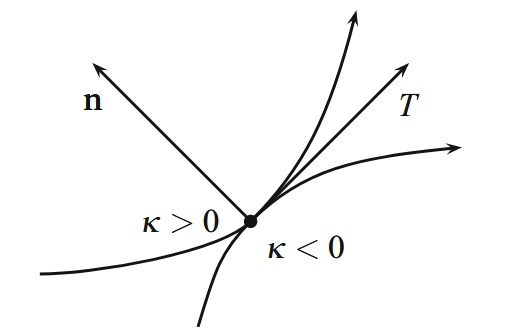
\includegraphics[width=0.4\textwidth]{../Lectures/Figures/curvature.png}
    \caption{The sign of the curvature~\cite[p.~12]{tuDifferentialGeometry2017}.}
\end{figure}
\begin{example}
    Recall Example~\ref{eg. circle}, we can easily compute 
    \begin{align}
        T'=[-\frac{1}{a}\cos\frac{s}{a}, -\frac{1}{a}\sin\frac{s}{a}]^\top, \nonumber
    \end{align}
    the normal vector $\vn={[-\cos\frac{s}{a}, -\sin\frac{s}{a}]}^\top$.
    So the curvature $\kappa=\frac{1}{a}$.
\end{example}
\subsection{Orientation and Curvature}
For a arc length parameterized curve that the two endpoints are fixed, 
will have two parameterization that inverse the orientation. Let the arc length be $\ell$,
then, we have another parameterization by
\begin{align}
    \tilde{\gamma}(s)=\gamma(\ell - s). \nonumber
\end{align}
Then, the velocity and its derivative give
\begin{align}
    \tilde{T}(s)=-T(\ell - s), \quad \tilde{T}'(s)=T'(\ell - s). \nonumber
\end{align}
The unit norm vector is given by rotate $\tilde{T}(s)$ by $\frac{\pi}{2}$
\begin{align}
    \tilde{\vn}(s)=\text{rot}\left(\frac{\pi}{2}\right)\tilde{T}(s)
    =-\text{rot}\left(\frac{\pi}{2}\right)T(\ell - s)=-\vn(\ell - s). \nonumber
\end{align}
The sign of curvature will be reversed by
\begin{align}
    \tilde{\kappa}(s)=\inner{\tilde{\vn}(s)}{\tilde{T}'(s)}
    =\inner{-\vn(\ell - s)}{T'(\ell - s)}=-\kappa(\ell-s). \nonumber
\end{align}
\begin{example}
    From Example~\ref{eg. circle}, the clockwise circle has the signed curvature $-1/a$.
\end{example}
\begin{figure}[htb]
    \centering
    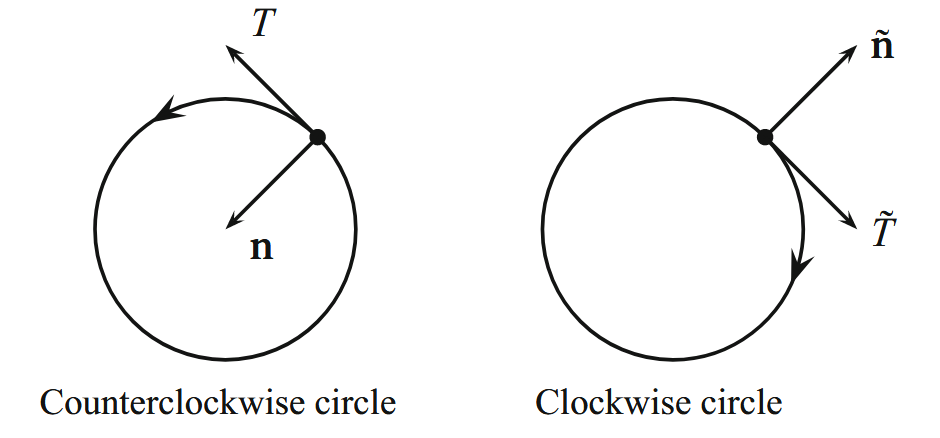
\includegraphics[width=0.7\textwidth]{../Lectures/Figures/reverse_orient.png}
    \caption{Reverse of a curve and its curvature~\cite[p.~13]{tuDifferentialGeometry2017}.}
\end{figure}
\problemsection{Problems}
\begin{problem}
    Let $T(s)$ be the unit tangent vector field on a plane curve $\gamma(s)$ parametrized 
    by arc length. Write
\[
T(s) = \begin{bmatrix}
        \cos \theta(s) \\ 
        \sin \theta(s) 
        \end{bmatrix},
\]
where $\theta(s)$ is the angle of $T(s)$ with respect to the positive horizontal axis. 
Show that the \textbf{signed curvature} $\kappa$ is the derivative $d\theta/ds$.
\label{problem. 2.1}
\end{problem}

\begin{problem}
    In physics literature, it is customary to denote the derivative with respect to time by a dot,
    e.g., $\dot{x} = dx/dt$, and the derivative with respect to distance by a prime, 
    e.g., $x' = dx/ds$. We will sometimes follow this convention.
    Let $c(t) = (x(t), y(t))$ be a regular plane curve. 
    Using Problem~\ref{problem. 2.1} and the chain rule 
    $d\theta/ds = (d\theta/dt)/(ds/dt)$, 
    show that the signed curvature of the curve $c(t)$ is
\[
\kappa = \frac{\dot{x}\ddot{y} - \dot{y}\ddot{x}}{(\dot{x}^2 + \dot{y}^2)^{3/2}},
\]
where $\dot{x} = dx/dt$ and $\ddot{x} = d^2x/dt^2$.
\end{problem}

\begin{problem}
    The \emph{graph} of a $C^\infty$ function $y = f(x)$ is the set
\[
\left\{ (x, f(x)) \mid x \in \mathbb{R} \right\}
\]
in the plane. Show that the signed curvature of this graph at $(x, f(x))$ is
\[
\kappa = \frac{f''(x)}{\left(1 + \left(f'(x)\right)^2\right)^{3/2}}.
\]
\end{problem}

\begin{problem}
    The ellipse with equation $x^2/a^2 + y^2/b^2 = 1$ in the $(x,y)$-plane (Figure~2.4) 
    can be parametrized by
\[
x = a\cos t, \quad y = b\sin t, \quad 0 \leq t \leq 2\pi.
\]
Find the curvature of the ellipse at an arbitrary point $(x,y)$.
\end{problem}

\begin{problem}
    Let $I$ be a closed interval in $\mathbb{R}$. If $\gamma \colon I \to \mathbb{R}^3$ is
     a regular space curve parametrized by arc length, 
     its \emph{curvature} $\kappa$ at $\gamma(s)$ is defined to be 
     $\|\gamma''(s)\|$.\footnote{The curvature of a space curve is always nonnegative,
      while the signed curvature of a plane curve could be negative.
       To distinguish the two for a space curve that happens to be a plane curve, 
       one can use $\kappa_2$ for the signed curvature. 
       We will use the same notation $\kappa$ for both, 
     as it is clear from the context what is meant.} 
     Consider the helix $c(t) = (a\cos t, a\sin t, bt)$ in space.

\begin{enumerate}
    \item[(a)] Reparametrize $c$ by arc length: $\gamma(s) = c(t(s))$.
    \item[(b)] Compute the curvature of the helix at $\gamma(s)$.
\end{enumerate}
\end{problem}